\RequirePackage{expl3}
\ExplSyntaxOn
\cs_if_exist:NF \prop_gput_if_not_in:Nnn {
  \cs_gset_eq:NN \prop_gput_if_not_in:Nnn \prop_gput_if_new:Nnn
}
\ExplSyntaxOff

%%%%%%%%%%%%%%%%%%%%%%%%%%%%%%%%%%%%%%%
% PlushCV - One Page Two Column Resume
% LaTeX Template
% Version 1.0 (11/28/2021)
%
% Author:
% Shubham Mazumder (http://mazumder.me)
%
% Hacked together from:
% https://github.com/deedydas/Deedy-Resume
%
% IMPORTANT: THIS TEMPLATE NEEDS TO BE COMPILED WITH XeLaTeX
%
% 
%%%%%%%%%%%%%%%%%%%%%%%%%%%%%%%%%%%%%%
% 
% TODO:
% 1. Figure out a smoother way for the document to flow onto the next page.
% 3. Add more icon options 
% 4. Fix hacky left alignment on contact line
% 5. Remove Hacky fix for awkward extra vertical space
% 
%%%%%%%%%%%%%%%%%%%%%%%%%%%%%%%%%%%%%%
%
% CHANGELOG:
%
%%%%%%%%%%%%%%%%%%%%%%%%%%%%%%%%%%%%%%%
%
% Known Issues:
% 1. Overflows onto second page if any column's contents are more than the vertical limit.
%%%%%%%%%%%%%%%%%%%%%%%%%%%%%%%%%%%%%%
%%Icons:
%%Main: https://icons8.com/icons/carbon-copy
%%%%%%%%%%%%%%%%%%%%%%%%%%%%%%%%%%

\documentclass[]{plushcv}
\usepackage{fancyhdr}
\usepackage{tikz}
\pagestyle{fancy}
\fancyhf{}
\hyphenpenalty=10000

\begin{document}

%%%%%%%%%%%%%%%%%%%%%%%%%%%%%%%%%%%%%%
%
%     TITLE NAME
%
%%%%%%%%%%%%%%%%%%%%%%%%%%%%%%%%%%%%%%
\vspace*{1mm}
\noindent\begin{minipage}[t]{0.17\textwidth}
  \vspace{0pt}
  \begin{tikzpicture}
    \clip (0,0) circle (1.5cm);
    \node at (0,-0.2) {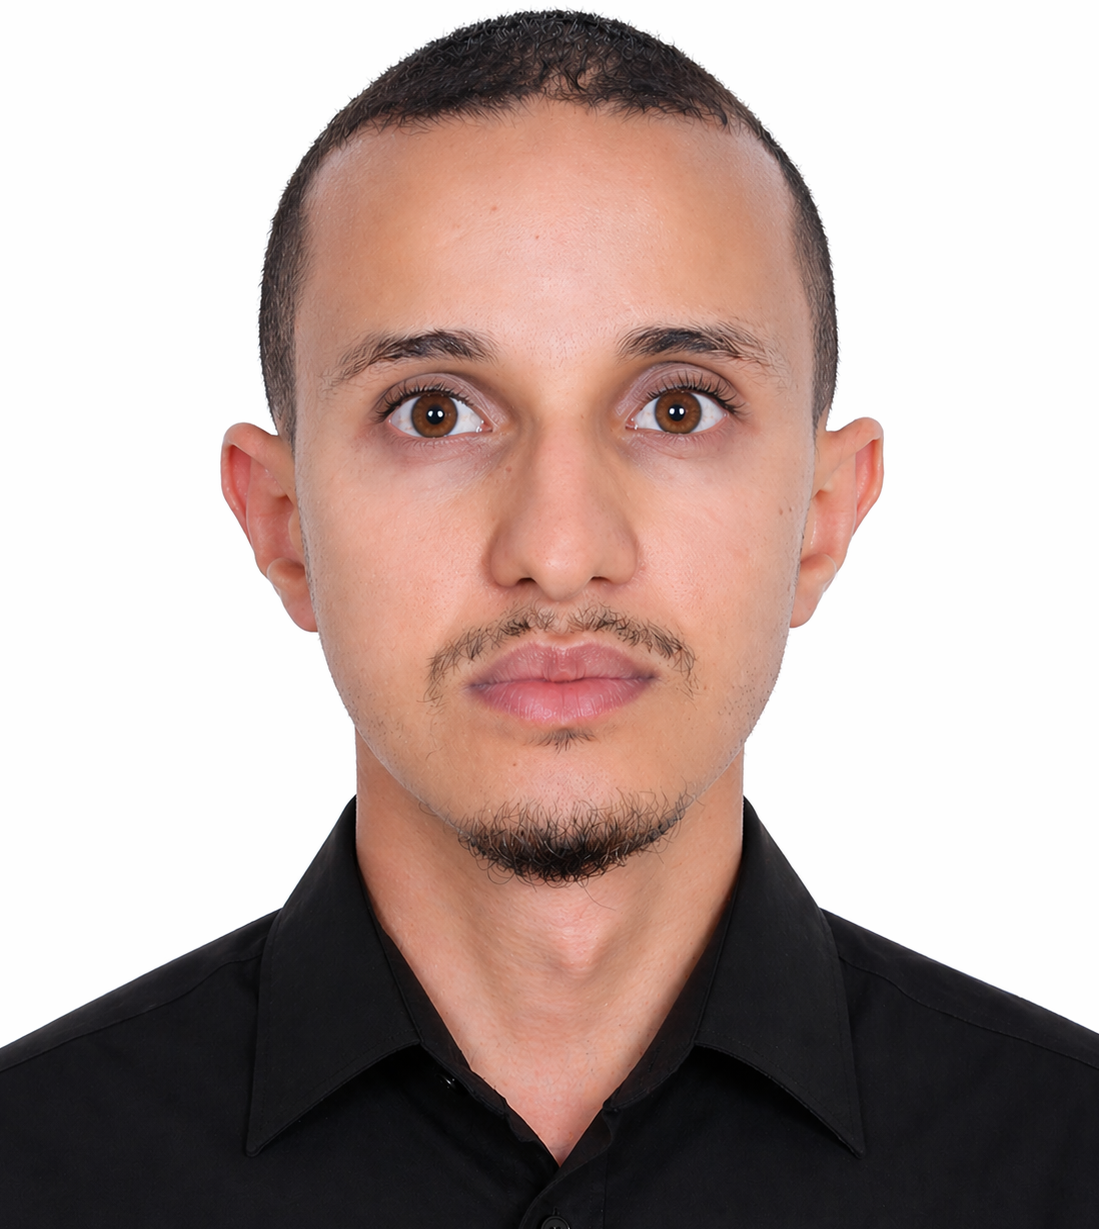
\includegraphics[width=3.2cm]{assets/imageee.png}};
  \end{tikzpicture}
\end{minipage}%
\hspace{0.05cm}
\begin{minipage}[t]{0.78\textwidth}
\namesection{Izelmadene}{Achraf}
{  \normalsize Élève Ingénieur en Génie Électrique et Systèmes Intelligents}
%Futur Ingénieur
{\contactline{\href{https://www.linkedin.com/in/achraf-izelmadene/}
{ACHRAF IZELMADENE}}
{\href{mailto:achraf.izelmadene@gmail.com}
{achraf.izelmadene@gmail.com}}
{\href{tel:+212699098736}
{+212699098736}}}
\end{minipage}
\vspace{0.1em}
\begin{minipage}[t]{0.72\textwidth} 


%%%%%%%%%%%%%%%%%%%%%%%%%%%%%%%%%%%%%%
%     À propos
%%%%%%%%%%%%%%%%%%%%%%%%%%%%%%%%%%%%%%

\section{À propos de moi}
%\small
Étudiant en 4ᵉ année de Génie Électrique et Systèmes Intelligents \`a l'EMSI, passionné par l'innovation technologique, les systèmes embarqués et l'IoT. Toujours à la recherche de nouveaux défis pour appliquer mes compétences techniques et concevoir des solutions intelligentes.
\sectionsep
%\vspace{5mm}
\section{Education}
\runsubsection{Diplôme d'ingénieur en Électrique et Systèmes Intelligents}
\descript{École Marocaine des Sciences de l'Ingénieur \textbf{(EMSI)}}\hfill\location{2025 - Présent}

%\vspace{\topsep} % Hacky fix for awkward extra vertical spacetc.
%\end{tightemize}
\sectionsep
\runsubsection{Licence en Sciences de la Mati\`ere Physique  \space \small\textit{Option: Automatique}} {}
%fondamentale
\descript{Faculté des Sciences Semlalia de Marrakech \textbf{(FSSM)}}\hfill\location{2020-2024}

\sectionsep
\runsubsection{Baccalauréat Sciences Physiques (PC)}
\descript{ Lycée Al Maghrib Al Arabi Marrakech}\hfill\location{2020}
\sectionsep
%%%%%%%%%%%%%%%%%%%%%%%%%%%%%%%%%%%%%%
%     Experience
%%%%%%%%%%%%%%%%%%%%%%%%%%%%%%%%%%%%%
\section{Experience}
\runsubsection{Stagiaire en unité de production }

\descript{Ménara Préfa}\hfill\location{ JUL 2024}
\vspace{\topsep} % Hacky fix for awkward extra vertical space
\begin{tightemize}
\sectionsep
\item Stage d'un mois à Ménara Préfa au sein de l'unité de production.
\item Réalisation d'un projet de migration d'un automate vers un Siemens.
\item Développement des compétences en maintenance industrielle et en production.  
\end{tightemize}
%%%%%%%%%%%%%%%%%%%%%%%%%%%%%%%%%%%%%%%%%%%%%%%%%%%%%%%%%%%%%%%%%%%%%%%%%%%%


\section{Projets}

\runsubsection{Smart Agriculture IoT Ecosystem}
\vspace{\topsep}
\begin{tightemize}
\item Écosystème IoT d'irrigation intelligente orchestrant des nœuds capteurs (Arduino Nano + LoRa) et une unité centrale de décision (ESP32 + logique floue), avec dashboard de monitoring temps réel et modèle TFLite embarqué pour la détection de maladies foliaires.
\end{tightemize}
\sectionsep

\runsubsection{Maintenance Prédictive 4.0 par AutoML}
\vspace{\topsep}
\begin{tightemize}
\item Comparaison TPOT vs. Auto-WEKA sur données IoT industrielles (vibrations, température) pour détection anticipée de défaillances moteur, avec analyse de data leakage et validation croisée temporelle.
\end{tightemize}
\sectionsep

\runsubsection{Simulation d'un bras robotique (jeu d'échecs)}
\vspace{\topsep}
\begin{tightemize}
\item Modèle 3D SolidWorks, import URDF et simulation PyBullet avec cinématique inverse pour le contrôle des mouvements pièce par pièce.
\end{tightemize}
\sectionsep

\runsubsection{Traduction ASL par vision artificielle temps réel}
\vspace{\topsep}
\begin{tightemize}
\item Extraction de landmarks (MediaPipe), classification par ensemble learning (Random Forest + SVM + MLP) et traduction temps réel avec overlay vidéo.
\end{tightemize}
\sectionsep

\runsubsection{Détection d'anomalies Smartgrid (clustering)}
\vspace{\topsep}
\begin{tightemize}
\item Comparaison KMeans / DBSCAN / GMM sur données IoT smartgrid ; évaluation Precision/Recall, silhouette score et dashboard de visualisation des clusters.
\end{tightemize}
\sectionsep

\runsubsection{Voiture télécommandée Arduino}
\vspace{\topsep}
\begin{tightemize}
\item Commande différentielle des moteurs DC via module RF et évitement d'obstacles par capteur ultrasonique.
\end{tightemize}
\vspace{-3pt}

%%%%%%%%%%%%%%%%%%%%%%%%%%%%%%%%%%%%%%
%
%     COLUMN TWO
%
%%%%%%%%%%%%%%%%%%%%%%%%%%%%%%%%%%%%%%

\end{minipage} 
\hfill
\begin{minipage}[t]{0.24\textwidth} 

%%%%%%%%%%%%%%%%%%%%%%%%%%%%%%%%%%%%%%
%     SKILLS
%%%%%%%%%%%%%%%%%%%%%%%%%%%%%%%%%%%%%%
\section{Skills}
\sectionsep
\vspace{2pt}

\subsection{Programming}
\sectionsep
C/C++ \textbullet{} Python \textbullet{}\\ JavaScript \textbullet{} HTML/CSS
\sectionsep
\vspace{2pt}

\subsection{LOGICIELS}
\sectionsep
MATLAB \textbullet{} SIMULINK \textbullet{} \\Caneco BT \textbullet{} TIA PORTAL \textbullet{} RSView \textbullet{} 
SolidWorks \textbullet{} TinkerCAD  \textbullet{} 
Pack Office \\(Word, Excel, PowerPoint)
\vspace{2pt}

\sectionsep
\subsection{Tools/Platforms}
\sectionsep
Git \textbullet{} Docker \textbullet{} PyBullet \\
Arduino \textbullet{} Supabase \textbullet{}\\ 3DEXPERIENCE \\
\sectionsep

%%%%%%%%%%%%%%%%%%%%%%%%%%%%%%%%%%%%%%
%     EDUCATION
%%%%%%%%%%%%%%%%%%%%%%%%%%%%%%%%%%%%%%
\vspace{4pt}
\section{CERTIFICATIONS}
\sectionsep

\subsection{3DEXPERIENCE Collaborative \\ Industry Innovator}
\descript{Dassault Systèmes}
\vspace*{2pt}

\subsection{Sensors and Sensor Circuit Design}
\descript{Univ. of Colorado Boulder | Coursera}
\vspace*{2pt}

\subsection{Machine Learning in Production}
\descript{DeepLearning.AI | Coursera}
\vspace*{2pt}

\subsection{Foundations of IoT Systems}
\descript{LearnQuest | Coursera}
\sectionsep
\vspace{2pt}
\section{Awards}
\begin{tabular}{@{}p{0.5cm} p{3.8cm}}
\textbf{\large 1st} & \textbf{Hack The Intelligence} \\
 & {\footnotesize AISEC Int'l Summit \textbf{2026}} \\[4pt]
\textbf{\large 2nd} & \textbf{Vision AI Competition} \\
 & {\footnotesize EMSI Marrakech \textbf{2026}} \\
\end{tabular}
\sectionsep
\vspace{0.5pt}
\section{Languages}
\vspace{2pt}

\begin{flushleft}
 \textbullet{} Arabic (maternelle) \\ \textbullet{} Français (DELF B2) \\ \textbullet{} Anglais (EFSET B2)
\end{flushleft}
\vfill

\end{minipage} 
\end{document}
